\section{High-Performance Computing with \GAP}\label{sec:hpc}

Experiments with parallel computing in \GAP date back to the late
1990s. The {\sf ParGAP} package by Gene Cooperman and others \cite{pargap}
implemented a limited set of MPI bindings and experimented with a
number of variations of the master--worker paradigm. It was not
widely adopted due, we believe, to a lack of suitable clusters available to typical
\GAP users at the time, and issues with robustness, installation and
debugging support.

Within the Framework 6 project SCIEnce: Symbolic Computation
Infrastructure for Europe, we developed the SCSCP package \cite{SCSCP}, which
provided a much more robust remote procedure call architecture for
\GAP which still serves a variety of uses, including effective support
for coarse-grained distributed memory parallel computation, suitable
for a cloud or \textit{ad hoc} cluster environment, as seen for
example, in \cite{loughlin}. Compared to MPI, it is much less
efficient, but much more fault-tolerant and more adaptable to
heterogeneous environments.

In this project, we have therefore focused our attention on shared
memory parallelisation, relevant to many of our users given that even
modern laptops may have up to six cores, while 64 core servers or
cloud nodes are widely available to many research mathematicians.

\subsection{\HPCGAP: Multi-Threaded Programming in \GAP}\label{hpc-gap}

\GAP 4.9.1 (Month 33) for the first time included experimental code to 
support safe multi-threaded programming in \GAP, dubbed \HPCGAP. This
had been in development for some time as a fork of \GAP and the \HPCGAP and \GAP
codebases had diverged. In this release we reunified them,
making thread support a compile-time option instead of requiring a completely
different program. This was an essential step to support further development of
\HPCGAP, and ensure that new developments in \GAP could be quickly
incorporated. It also provided general \GAP users an opportunity to start to experiment 
with \HPCGAP, for which documentation is also provided.

%\TODO{Remember to provide a copy of the HPC-GAP manual as an appendix}

\HPCGAP supports two models of parallel programming in \GAP, which can
be combined: threads and tasks. Threads operate as in most languages.
The basic primitive is to start execution of a \GAP function in a new
thread, while the calling thread returns immediately. Threads can
interact through global data, by passing interrupts or by returning
results when they exit. Thread-local variables are available as an
alternative to global variables.

Tasks are
similar, but a task is submitted to a shared job queue and executed by
one of a fixed-size pool of worker threads. Typically the calling
program will start a number of tasks and then wait for some or all
of them to complete, leaving the task scheduler to allocate each task
to a worker. A task can be scheduled to run only when another
has completed, and more complex dependencies can be expressed using
``milestones''.

A number of data structures and other features are provided to
simplify the programming of interactions between tasks and/or
threads. These were developed in consultation with a group of \GAP
developers, based on the specific types of computation that they
anticipated needing to parallelize. They include:
\begin{itemize}
\item Atomic lists and records, which behave like standard \GAP data
    structures, but guarantee that their basic access operations are
    thread-safe;
  \item Channels (efficient first-in-first-out data structures
    designed to pass objects between threads or tasks);
  \item Synchronization variables which guarantee that exactly one
    write to the variable will succeed; and
  \item Traditional semaphores.
\end{itemize}
Full details can be found in the \HPCGAP manual in Appendix~\ref{sec:hpc-manual}.

Implementing all of this efficiently required a substantial
refactoring of the \GAP interpreter, but presented no other challenges
unique to \GAP.  What does present a serious challenge for \HPCGAP, however, is that the \GAP
library makes very extensive use of shared global data, which is
frequently updated as new knowledge is obtained. Removing this sharing
of knowledge would make the overall system much less effective, as
well as requiring millions of lines of code to be rewritten, but
ensuring that access and updates to this data from different threads
and tasks do not cause corruption or inconsistency was difficult.

The approach taken was to limit access, in most cases, to
data ``owned'' by the accessing thread, read-only data and ``public''
data stored in thread-safe data structures which were used for the
global ``knowledge pool''. In particular, this last set of data could
be updated ``atomically'', so any thread would see the old state
\emph{or} the new one, but nothing in between. The access limitations are implemented by
access checks in the kernel, with the aim of ensuring that most unsafe
data access should result in error messages, rather than inconsistent
results. Experiments with this system have been reported in a number
of papers, for instance \cite{HPCGAP-paper}.

The main remaining challenge is to complete the adaptation of the
enormous legacy codebase represented by \GAP's library and key
packages to use these mechanisms effectively, and to keep the
underlying mechanisms working as the core \GAP codebase
evolves. Fusing the codebases, as was done in \GAP~4.9, was a critical
step in this work, meaning, for instance, that all changes to \GAP are
tested in \HPCGAP automatically.

The effectiveness of the underlying task mechanism is illustrated in
the graph in Figure \ref{fig:hpcgap-speedups}, which shows the speedups (wall-clock time on $n$
cores versus CPU time on one core) achieved in running 1000 test tasks
(each taking about 300ms) with various numbers of worker threads on a 64
core AMD ``bulldozer'' system. These cores share L2 cache and decode
hardware in pairs, limiting performance with larger numbers of
threads.

\begin{figure}[!ht]
    \centering
    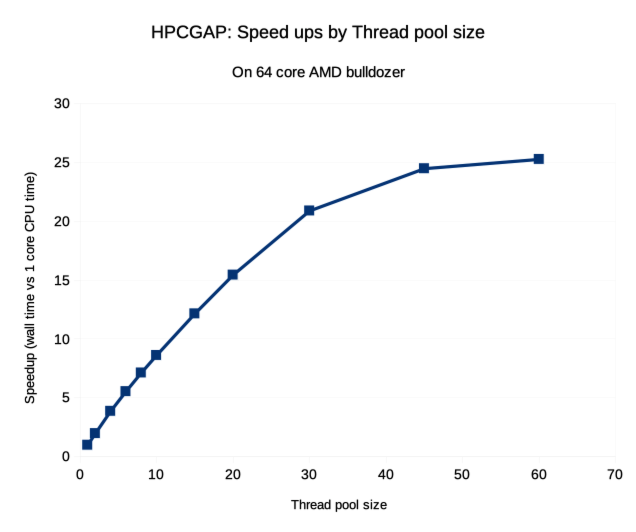
\includegraphics[width=0.8\textwidth]{images/hpcgap-speedups}
    \caption{Speedups achieved by HPCGAP on 1000 test tasks}\label{fig:hpcgap-speedups}
\end{figure}


% Release announcement: https://www.gap-system.org/Manuals/doc/changes/chap3.html#X7F52B77B7DBACC17

% \HPCGAP manual: https://www.gap-system.org/Manuals/doc/hpc/chap0.html

% What about making https://www.gap-system.org/Manuals/doc/hpc/manual.pdf 
% an electronic appendix to the deliverable?

\subsection{Meataxe64: High-Performance Linear Algebra over Finite Fields}\label{meataxe64}

A key kernel for many applications of \GAP is linear algebra for
mainly dense matrices over
a range of finite fields, especially small ones. This is used directly in working with
matrix groups and in computational representation theory, but also
arises indirectly in areas such as graph theory, finite solvable
groups and number theory. 

The \GAP kernel already includes memory-efficient
representations of matrices over these fields, and implementations
based on the C-meataxe (the name ``meataxe'' is derived from the
abbreviation ``mtx'' for ``matrix'' and the fact that a key operation
in computational representation theory is to ``chop'' a module into
its irreducible components).

Working with external collaborators (primarily R.~A.~Parker), we have
supported (and continue to contribute to) the design and development
of a new C and assembler library, called ``meataxe64'', which takes
advantage of new algorithmic ideas, and of powerful features of modern
CPUs, to deliver a quantum leap in performance for matrix
multiplication and Gaussian elimination on modern multi-core shared
memory computers. This project has involved radical innovations in
low-level data formats and arithmetic algorithms, in cache-friendly
loop structures (similar to those now standard in BLAS implementations,
but made more complex by the need to reorganize and reformat both
inputs and outputs of a multiplication), in matrix level reduction
algorithms (both for non-prime fields of all characteristics, inspired
by Albrecht \cite{m4rie}, and along Strassen-Winograd lines), in a
very efficient dataflow-driven thread farm and in high-level
algorithms, especially for Gaussian elimination. A number of
publications are in preparation.

We have implemented a \GAP interface to this C library (the
``meataxe64 \GAP package'' \cite{meataxe64}) currently in beta-testing,
and are in the process of revising higher levels of the software stack
to make best use of it.

The meataxe64 C library is multi-threaded using a bespoke and
effective thread-farm that supports a powerful dataflow module of
computation. With this, the library can efficiently make
use of multiple cores for large enough matrices, whether used from
\HPCGAP or single-threaded \GAP. Particular care is taken to limit the use of
shared caches and of memory bandwidth in each task, so that they
interfere as little as possible. 

Tables \ref{fig:matmult:gap}, \ref{fig:matmult:mtx64} and
\ref{fig:matmult:par} indicate the performance gains and
speedups obtained by meataxe64 compared to our existing code.  The
data is based on run-times for multiplication of two random dense
square matrices of the given dimension with entries from $GF(q)$. In
these tables the throughput is calculated as the cube of the dimension
divided by the elapsed (``wall-clock'') time, ignoring algorithmic
techniques that may reduce the actual number of field operations
needed. The unit (Gfop/s) is billions of field operations per
second. 


\begin{small}
\begin{center}  
  \begin{longtable}{|c|c|c|c|c|}
\caption[]{Performance of existing \GAP code}\label{fig:matmult:gap}\\
    \hline
    $q$&Dim.&cpu (s)&wall (s) &throughput\\
    &&&& (Gfop/s)\\
    \hline
    \endfirsthead
\caption[]{Performance of existing \GAP code}\\
    \hline
    $q$&Dim.&cpu (s)&wall (s) &throughput\\
    &&&& (Gfop/s)\\
    \hline
    \endhead
    \hline
    \endfoot
2&800&0.004&0.003&149.6\\
2&1600&0.016&0.016&255.8\\
2&4000&0.159&0.159&401.7\\
2&8000&1.581&1.582&323.6\\
2&16000&14.241&14.280&286.8\\
2&40000&193.251&193.524&330.7\\
3&500&0.053&0.052&2.4\\
3&1000&0.364&0.364&2.8\\
3&2500&5.268&5.268&3.0\\
3&5000&41.529&41.533&3.0\\
3&10000&327.798&328.121&3.0\\
3&25000&5020.887&5025.466&3.1\\
4&400&0.017&0.017&3.8\\
4&800&0.112&0.112&4.6\\
4&2000&1.542&1.542&5.2\\
4&4000&12.107&12.108&5.3\\
4&8000&99.259&99.361&5.2\\
4&20000&1513.64&1515.528&5.3\\
5&300&0.021&0.021&1.3\\
5&600&0.147&0.148&1.5\\
5&1500&2.166&2.166&1.6\\
5&3000&17.106&17.108&1.6\\
5&6000&136.714&136.840&1.6\\
5&15000&2088.063&2089.934&1.6\\
7&200&0.009&0.009&0.9\\
7&400&0.063&0.062&1.0\\
7&1000&0.906&0.906&1.1\\
7&2000&7.32&7.321&1.1\\
7&4000&56.659&56.710&1.1\\
7&10000&875.08&875.901&1.1\\
16&200&0.007&0.007&1.2\\
16&400&0.044&0.044&1.4\\
16&1000&0.644&0.643&1.6\\
16&2000&4.978&4.978&1.6\\
16&4000&39.757&39.798&1.6\\
16&10000&628.858&629.651&1.6\\
17&100&0.003&0.003&0.4\\
17&200&0.018&0.018&0.4\\
17&500&0.273&0.273&0.5\\
17&1000&2.153&2.154&0.5\\
17&2000&17.119&17.131&0.5\\
17&5000&268.032&268.267&0.5\\
64&100&0.002&0.002&0.5\\
64&200&0.012&0.013&0.6\\
64&500&0.186&0.186&0.7\\
64&1000&1.448&1.448&0.7\\
64&2000&11.548&11.558&0.7\\
64&5000&294.897&297.453&0.4\\
81&100&0.003&0.003&0.4\\
81&200&0.019&0.019&0.4\\
81&500&0.284&0.284&0.4\\
81&1000&2.215&2.215&0.5\\
81&2000&21.285&21.353&0.4\\
81&5000&276.045&276.503&0.5\\
101&100&0.003&0.003&0.3\\
101&200&0.021&0.020&0.4\\
101&500&0.295&0.295&0.4\\
101&1000&2.287&2.287&0.4\\
101&2000&18.212&18.233&0.4\\
101&5000&321.134&322.902&0.4\\
  \end{longtable}
\end{center}

\begin{center}
  \begin{longtable}{|c|c|c|c|c|}
    \caption[]{Performance of Meataxe64 on one core}\label{fig:matmult:mtx64}\\
    \hline
    $q$&Dim.&cpu (s)&wall (s) &throughput\\
    &&&&(Gfop/s)\\
    \hline
    \endfirsthead
    \caption[]{Performance of Meataxe64 on one core}\\
    \hline
    $q$&Dim.&cpu (s)&wall (s) &throughput\\
    &&&&(Gfop/s)\\
    \hline
    \endhead
    \hline
    \endfoot
2&8000&0.478&0.490&1045.1\\
2&16000&3.476&3.541&1156.7\\
2&40000&47.125&47.713&1341.4\\
2&80000&327.569&331.744&1543.4\\
2&160000&3460.336&3522.279&1162.9\\
3&5000&0.566&0.578&216.3\\
3&10000&4.125&4.152&240.9\\
3&25000&56.788&56.971&274.3\\
3&50000&399.282&400.549&312.1\\
3&100000&2774.011&2798.002&357.4\\
4&4000&0.205&0.216&295.8\\
4&8000&1.475&1.480&346.0\\
4&20000&19.889&20.070&398.6\\
4&40000&140.18&141.497&452.3\\
4&80000&980.936&985.148&519.7\\
5&3000&0.585&0.588&45.9\\
5&6000&4.102&4.107&52.6\\
5&15000&53.351&53.394&63.2\\
5&30000&362.048&362.369&74.5\\
5&60000&2585.863&2589.959&83.4\\
7&2000&0.217&0.221&36.2\\
7&4000&1.541&1.545&41.4\\
7&10000&20.652&20.675&48.4\\
7&20000&145.626&145.854&54.8\\
7&40000&1014.896&1016.415&63.0\\
16&2000&0.085&0.089&89.7\\
16&4000&0.603&0.623&102.7\\
16&10000&8.538&8.625&115.9\\
16&20000&60.979&61.521&130.0\\
16&40000&426.445&430.764&148.6\\
17&1000&0.074&0.074&13.5\\
17&2000&0.51&0.510&15.7\\
17&5000&7.259&7.265&17.2\\
17&10000&50.043&50.081&20.0\\
17&20000&352.604&353.215&22.6\\
64&1000&0.034&0.038&26.0\\
64&2000&0.201&0.206&38.7\\
64&5000&2.57&2.604&48.0\\
64&10000&17.858&18.125&55.2\\
64&20000&125.306&127.344&62.8\\
81&1000&0.095&0.099&10.1\\
81&2000&0.492&0.497&16.1\\
81&5000&5.519&5.560&22.5\\
81&10000&39.363&39.592&25.3\\
81&20000&274.394&276.197&29.0\\
101&1000&0.107&0.108&9.3\\
101&2000&0.75&0.751&10.7\\
101&5000&10.374&10.385&12.0\\
101&10000&72.007&72.056&13.9\\
101&20000&507.043&507.795&15.8\\
  \end{longtable}
\end{center}
  
\begin{center}
  \begin{longtable}{|c|c|c|c|c|}
    \caption[]{Performance of Meataxe64 on 64 cores}\label{fig:matmult:par}\\
    \hline
    $q$&Dim.&cpu (s)&wall (s) &throughput\\
    &&&&(Gfop/s)\\
    \hline
    \endfirsthead
    \caption[]{Performance of Meataxe64 on 64 cores}\\
    \hline
    $q$&Dim.&cpu (s)&wall (s) &throughput\\
    &&&&(Gfop/s)\\
    \hline
    \endhead
    \hline
    \endfoot
2&80000&904.369&21.638&23662.2\\
2&160000&4638.836&151.735&26994.4\\
2&320000&33340.649&1040.551&31491.0\\
3&50000&1004.631&21.017&5947.6\\
3&100000&5443.318&196.317&5093.8\\
3&200000&39283.76&1201.458&6658.6\\
4&40000&355.516&10.157&6300.9\\
4&80000&2548.595&51.267&9987.0\\
4&160000&13560.306&538.945&7600.0\\
5&30000&974.333&18.874&1430.6\\
5&60000&6273.661&142.248&1518.5\\
5&120000&38362.156&1171.026&1475.6\\
7&20000&437.489&8.740&915.3\\
7&40000&3035.705&53.539&1195.4\\
7&80000&15050.673&465.735&1099.3\\
16&20000&89.048&7.138&1120.8\\
16&40000&1044.91&22.805&2806.4\\
16&80000&6212.503&202.530&2528.0\\
17&10000&141.266&2.999&333.4\\
17&20000&1001.397&17.793&449.6\\
17&40000&7038.438&123.414&518.6\\
64&10000&58.099&1.807&553.5\\
64&20000&342.525&8.892&899.6\\
64&40000&2310.548&45.095&1419.2\\
81&10000&120.235&2.640&378.7\\
81&20000&734.844&13.992&571.8\\
81&40000&4913.959&88.109&726.4\\
101&10000&216.491&4.269&234.3\\
101&20000&1508.308&26.374&303.3\\
101&40000&10572.959&182.572&350.5\\
  \end{longtable}
\end{center}
\end{small}

% Release is published last week. Added to the bibliography. -- AK
% Thanks. I'd like to add a release announcement somewhere. -- SL
